\documentclass{beamer}
\usefonttheme{serif}

\usepackage{silence}
% check out persiantex/bidi#20
\WarningFilter{biditools}{Patching `\enddocument' failed}

\usepackage{hyperref}

\usepackage{graphicx}
\graphicspath{{img}}

\newcommand{\titlefa}{%
طراحی کنترل‌کننده سیستم نورپردازی پیکسلی \lr{RGB} مبتنی بر برنامه کاربردی وب با رویکرد اینترنت اشیاء}

\newcommand{\authorfa}{محمدامین صامتی}

\newcommand{\rawsupervisorfa}{حامد خوش‌نیت}
\newcommand{\supervisorfa}{دکتر\space\rawsupervisorfa}

\newcommand{\departfa}{دانشکده مهندسی برق و کامپیوتر}

\newcommand{\instfa}{دانشگاه صنعتی اراک}

\newcommand{\datefa}{شهریور ۱۴۰۰}

\newcommand{\titleen}{Design of RGB Pixel System Controller based on Web Application with IoT Approach}

\newcommand{\authoren}{Mohammad Amin Sameti}

\newcommand{\supervisoren}{Dr. Hamed Khoshniyat}

\newcommand{\insten}{Arak University of Technology}

\newcommand{\dateen}{September 2021}


\usepackage{bookmark}

\usepackage{minted}
\setminted{fontsize=\scriptsize,breaklines,linenos,autogobble}

\usepackage{xepersian}
\settextfont{XB Niloofar}
\setlatintextfont{Liberation Serif}

\usepackage{beamer-rtl}

\mode<presentation>{}

\definecolor{background}{rgb}{.904,.975,1}
\setbeamercolor{background canvas}{bg=background}

\title{\titlefa}

\author{\authorfa}

\institute[\instfa]{%
	استاد راهنما:\\\textbf\supervisorfa\par%
	\vspace{2em}\departfa\\\instfa%
}

\date{\datefa}

\logo{\vspace{71mm}
\includegraphics[scale=.5]{arakut}}

\beamertemplatenavigationsymbolsempty
\setbeamertemplate{footline}{%
  \hfill\normalsize\vspace{0.7em}%
  \insertframenumber/\inserttotalframenumber%
  \hspace*{0.7em}%
}

\newcommand{\outline}{نگاه کلی}

\AtBeginSection[\outline]{%
  \begin{frame}<beamer>{\outline}
    \tableofcontents[currentsection]
  \end{frame}
}

\begin{document}

\begin{frame}
  \titlepage{}
\end{frame}

\section{سیستم‌های نورپردازی پیکسلی}
\subsection{کاربرد}

\begin{frame}{\subsecname}{\secname}
  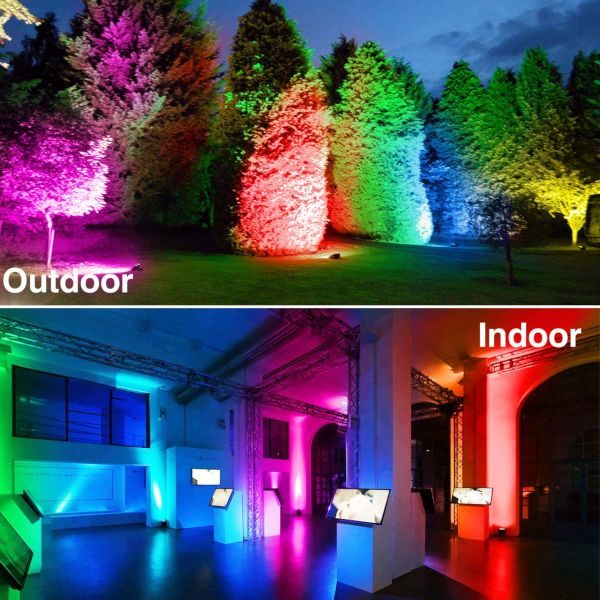
\includegraphics[scale=.15]{rgb-lighting}
\end{frame}

\subsection{اجزا}

\begin{frame}{\subsecname}{\secname}
  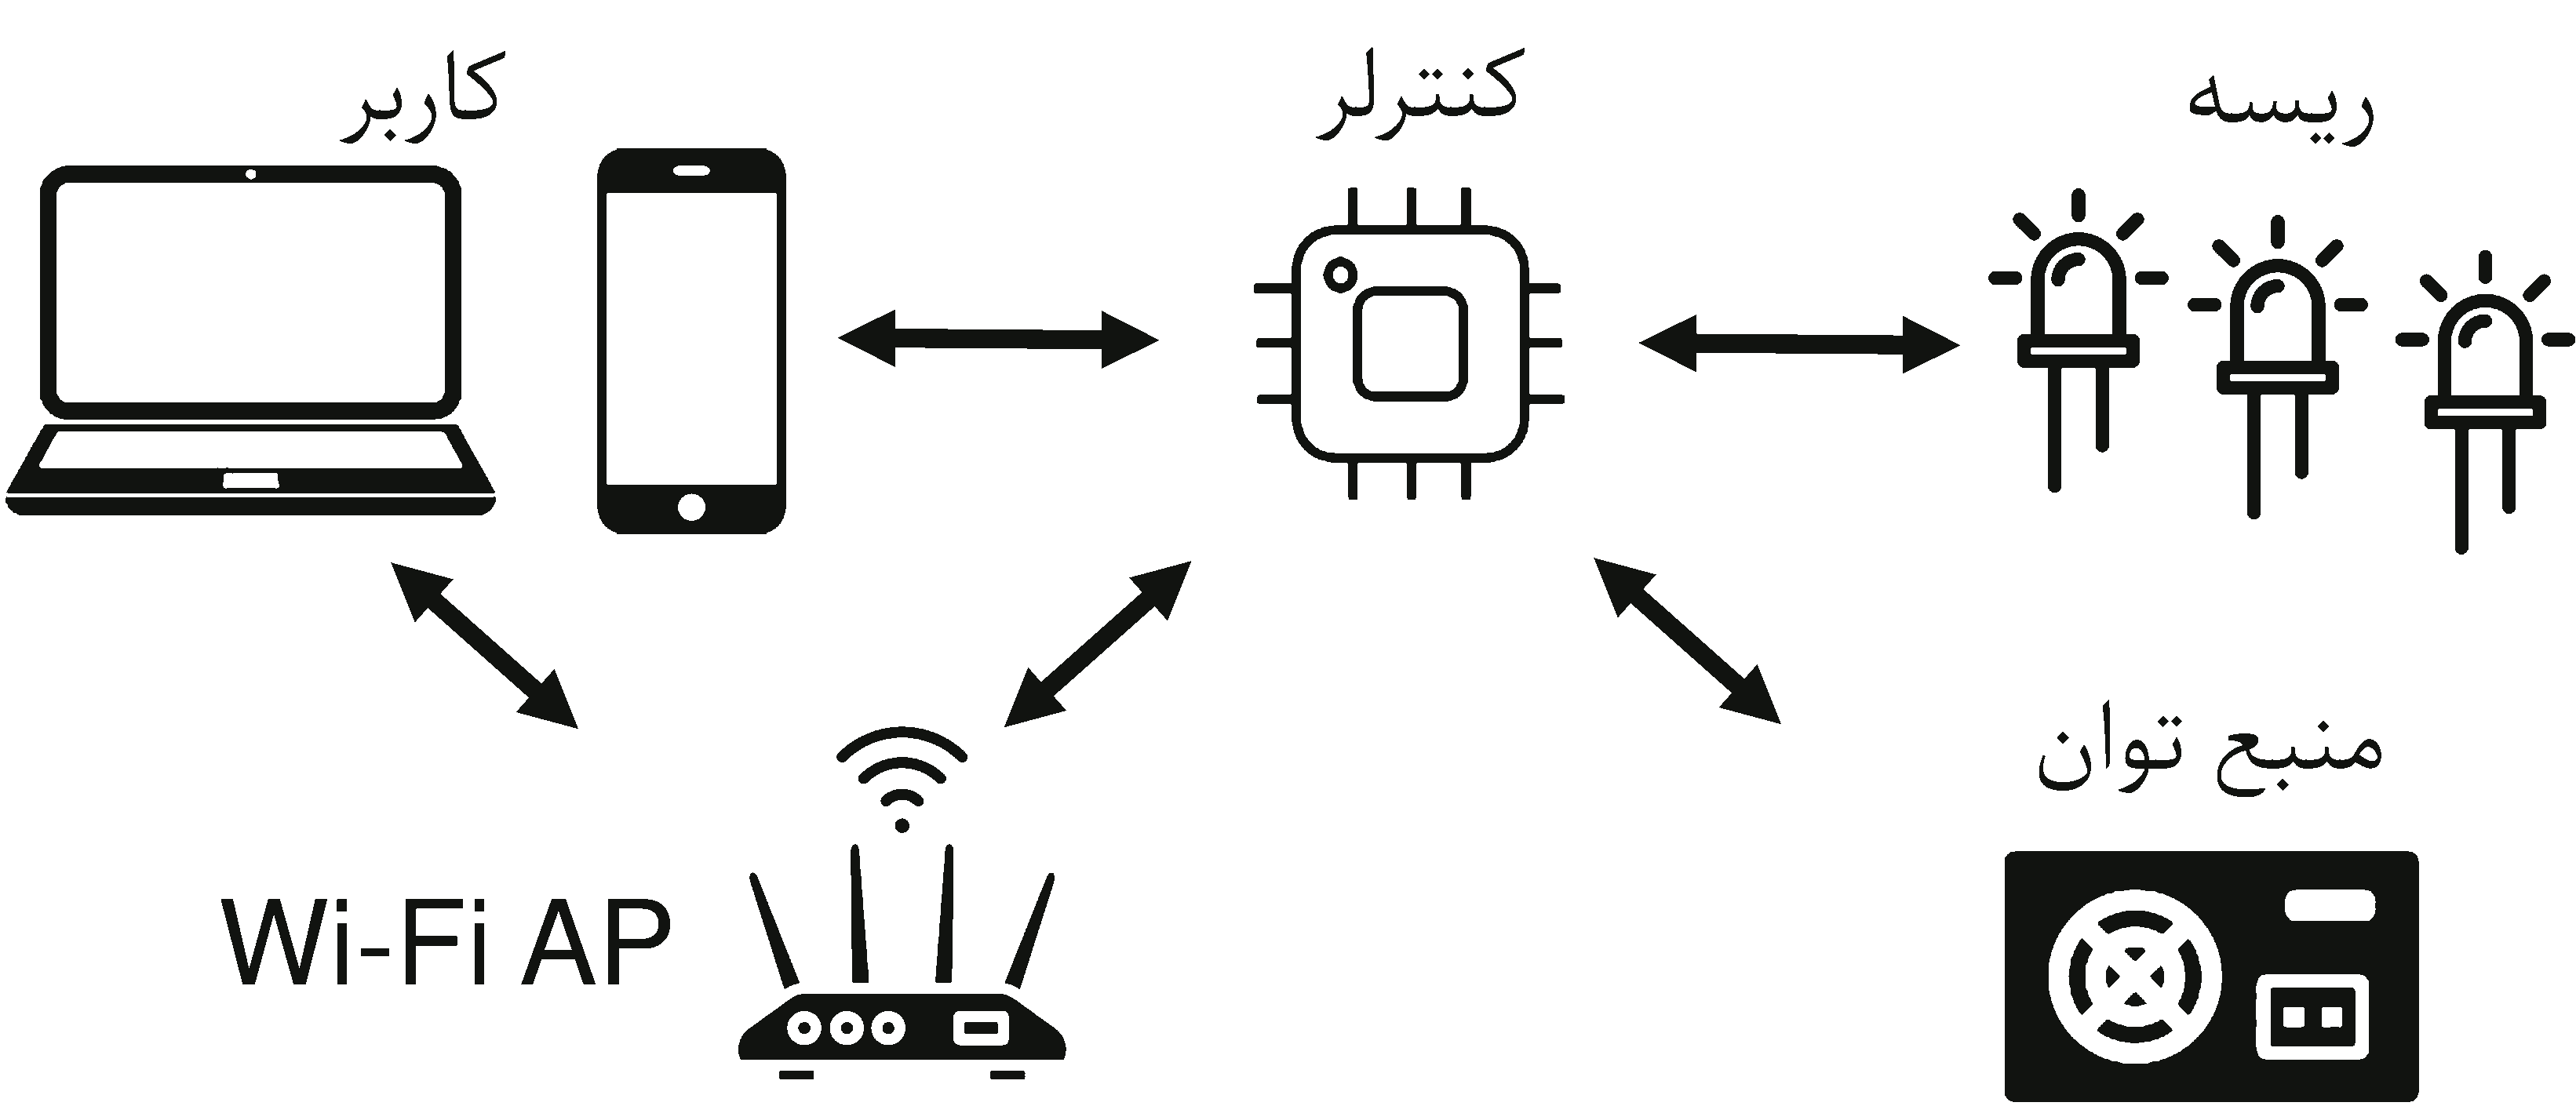
\includegraphics[scale=.35]{diagram2}
\end{frame}

\section{کنترلرها و بازار}
\subsection{اینترنت اشیاء}

\begin{frame}{\subsecname}{\secname}
  \begin{itemize}
    \item چیستی
    \item مزایا و معایب
    \item استفاده در این پروژه
  \end{itemize}
\end{frame}

\subsection{نمونه‌های موجود}

\begin{frame}{\subsecname}{\secname}
  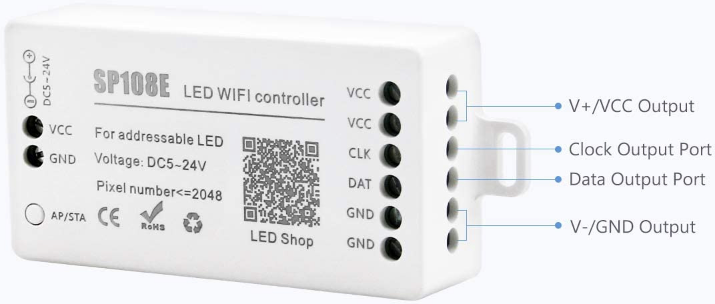
\includegraphics{controller}
\end{frame}

\begin{frame}{\subsecname}{\secname}
  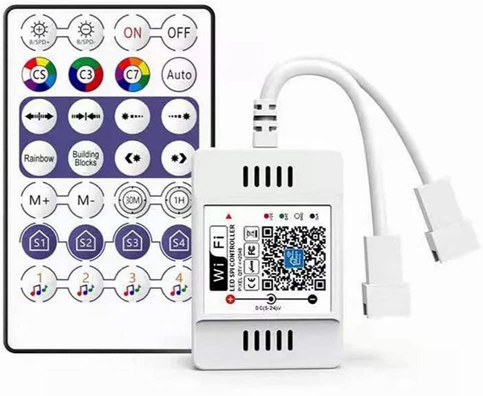
\includegraphics[scale=.9]{controller2}
\end{frame}

\section{ریسه‌های آدرس‌پذیر}

\subsection{کارکرد}

\begin{frame}{\subsecname}{\secname}
  \begin{columns}
    \column{.4\linewidth}%
      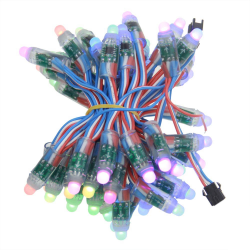
\includegraphics[width=\columnwidth]{ws2811}
    \column{.4\linewidth}%
      {\centering\textbf{ویژگی‌ها}\par}
      \vspace{1em}

      \begin{itemize}
        \item آدرس‌پذیری
        \item حافظه (فقط نوشتنی)
        \item تکی یا گروهی
        \item ایجاد توالی
      \end{itemize}
  \end{columns}
\end{frame}

\subsection{پروتکل}

\begin{frame}{\subsecname}{\secname}
  \textbf{اتصال الکتریکی}
  \vspace{1em}

  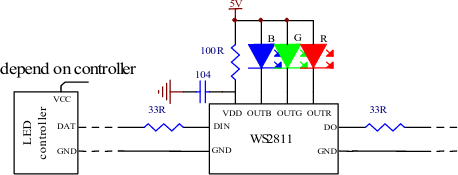
\includegraphics[scale=.6]{ws2811-wiring}
\end{frame}

\begin{frame}{\subsecname{}}{\secname}
  \textbf{برقراری ارتباط با ریسه}
  \vspace{1em}

  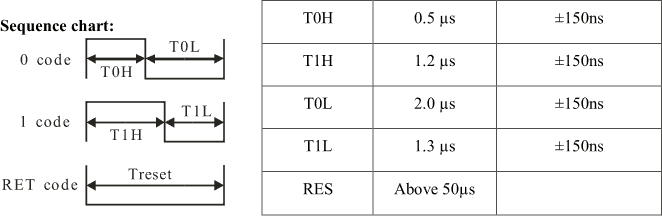
\includegraphics[scale=.63]{ws2811-pcm}
\end{frame}

\begin{frame}{\subsecname}{\secname}
  \textbf{ارتباط دیجیتالی}

  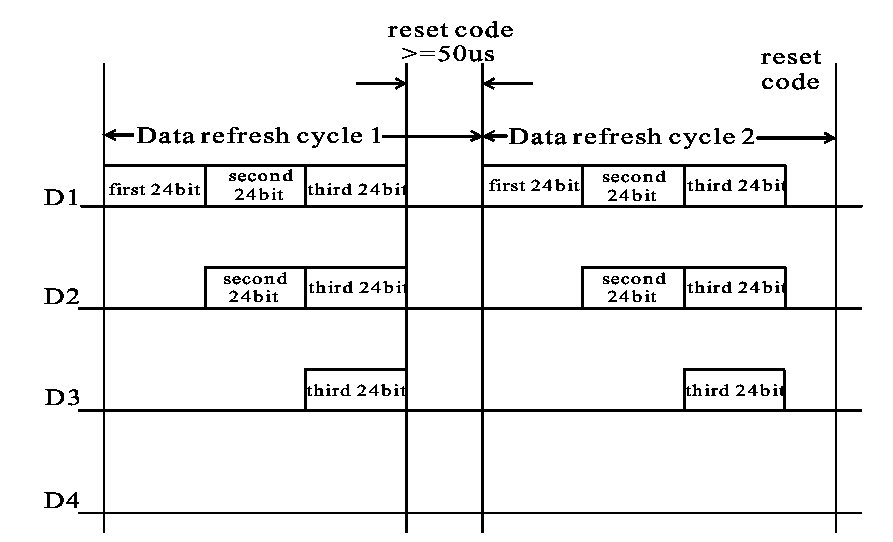
\includegraphics[scale=.34]{ws2811-proto}
\end{frame}

\section{پیاده‌سازی}
\subsection{سخت‌افزار}

\begin{frame}{\subsecname}{\secname}
  \textbf{نمای کلی}
  \vspace{1em}

  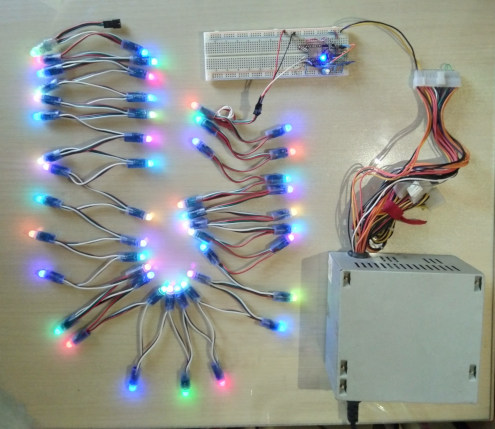
\includegraphics[scale=.9]{setup}
\end{frame}

\begin{frame}{\subsecname}{\secname}
  \textbf{کنترلر از نزدیک}
  \vspace{1em}

  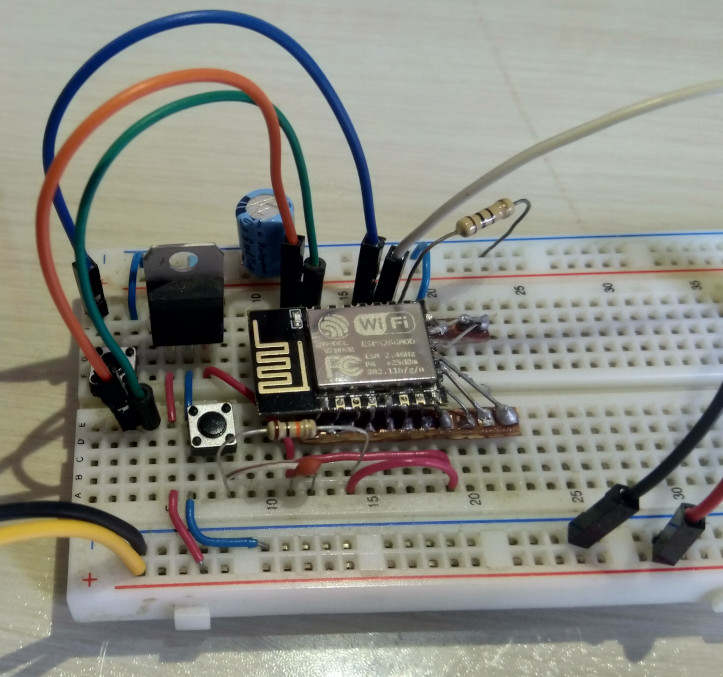
\includegraphics[scale=1.1]{close-up}
\end{frame}

\subsection{سفت‌افزار}

\begin{frame}{\subsecname}{\secname}
  \textbf{مراحل شروع به کار}

  \begin{enumerate}
    \item بوت کنترلر
    \item اتصال کاربر یا \lr{AP}
    \item بارگزاری برنامه کاربردی وب
    \item برقراری ارتباط با کنترلر
    \item ارسال فرمان
  \end{enumerate}
\end{frame}

\begin{frame}{\subsecname}{\secname}
  \textbf{سفت‌افزار به کار رفته}

  \begin{enumerate}
    \item کد نوشته شده
    \item WLED
  \end{enumerate}
\end{frame}

\begin{frame}{\subsecname{} نوشته شده}{\secname}
  \begin{columns}
    \column{.5\linewidth}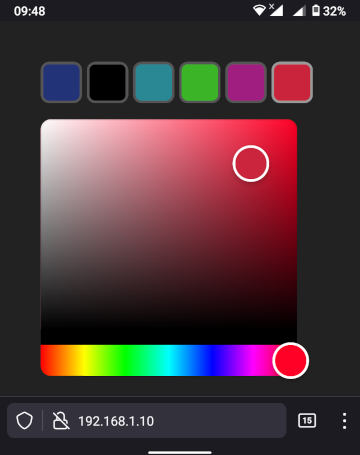
\includegraphics[width=\linewidth]{app}
    \column{.2\linewidth}\centering\textbf{رابط کاربری برنامه (مرورگر)}
  \end{columns}
\end{frame}

\newcommand{\LTRtriangle}{%
  \usebeamercolor[fg]{itemize item}
  {\vspace{1ex}\tiny$\blacktriangleright$}}

\begin{frame}{\subsecname{} نوشته شده}{\secname}
  \textbf{ابزارها و کتابخانه‌ها}

  \begin{LTR}
    {\LTRtriangle} PlatformIO (like CMake + PIP)

    {\LTRtriangle} Arduino Framework

    {\LTRtriangle} HTTP + WebSocket server
  \end{LTR}
\end{frame}

\begin{frame}{\subsecname{} نوشته شده}{\secname}
  \textbf{پروسه ساخت}
  \vspace{1em}

  \begin{enumerate}
    \item اضافه‌زدایی (\lr{Minification}) کد \lr{JS}
    \item فشرده‌سازی با \lr{G-Zip}
    \item تبدیل به آرایه در \lr{C}
    \item وارد کردن در کد سفت‌افزار
    \item کامپایل سفت‌افزار
  \end{enumerate}
\end{frame}

\begin{frame}{\subsecname{} نوشته شده}{\secname}
  \textbf{برقراری ارتباط با مرورگر}

  \begin{latin}
    \inputminted[firstline=20,lastline=28]%
    {C}{espws2811/src/main.cpp}
  \end{latin}

  \rule{\linewidth}{.4pt}

  \begin{latin}
    \inputminted[firstline=147,lastline=156]%
    {jsx}{espws2811/web/index.jsx}
  \end{latin}
\end{frame}

\begin{frame}{\subsecname{} نوشته شده}{\secname}
  \textbf{خروجی \lr{UART} معکوس شده (شبه \lr{PCM})}
  \vspace{1em}

  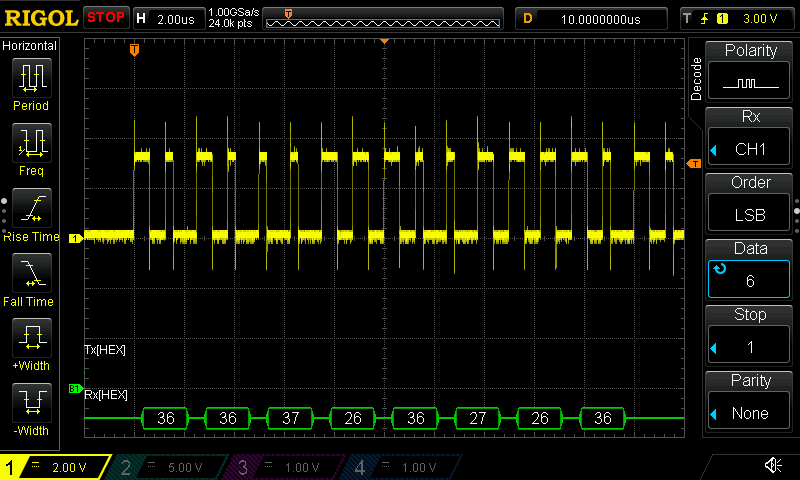
\includegraphics[width=\linewidth]{scope}
\end{frame}

\begin{frame}{\subsecname{} نوشته شده}{\secname}
  \textbf{برقراری ارتباط با ریسه}

  \begin{latin}
    \inputminted[firstline=40,lastline=48]%
    {C}{espws2811/src/ws2811.c}
  \end{latin}

  \begin{latin}
    \inputminted[firstline=15,lastline=21]%
    {C}{espws2811/src/ws2811.c}
  \end{latin}
\end{frame}

\begin{frame}{\subsecname{} \lr{WLED}}{\secname}
  \begin{columns}
    \column{.3\linewidth}%
      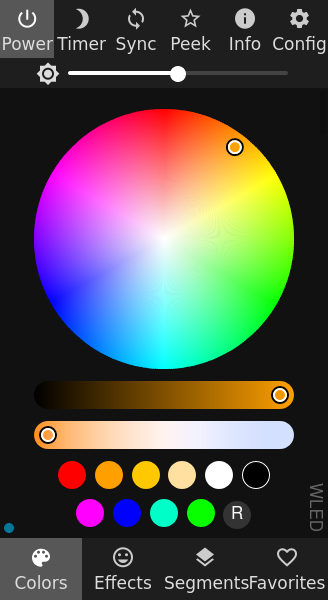
\includegraphics[width=\columnwidth]{wled}
    \column{.4\linewidth}%
      \textbf{علل انتخاب \lr{WLED}}
      \vspace{1em}

      \begin{itemize}
        \item متن‌باز
        \item تنوع پروتکل ریسه‌ها
        \item طول پویا و قابل تنظیم
        \item افکت‌های مختلف
        \item فرمان‌پذیری روی \lr{UDP}
      \end{itemize}
  \end{columns}
\end{frame}


\subsection{نرم‌افزار}

\begin{frame}{\subsecname}
  \textbf{\lr{LEDFX}}
  \vspace{1em}

  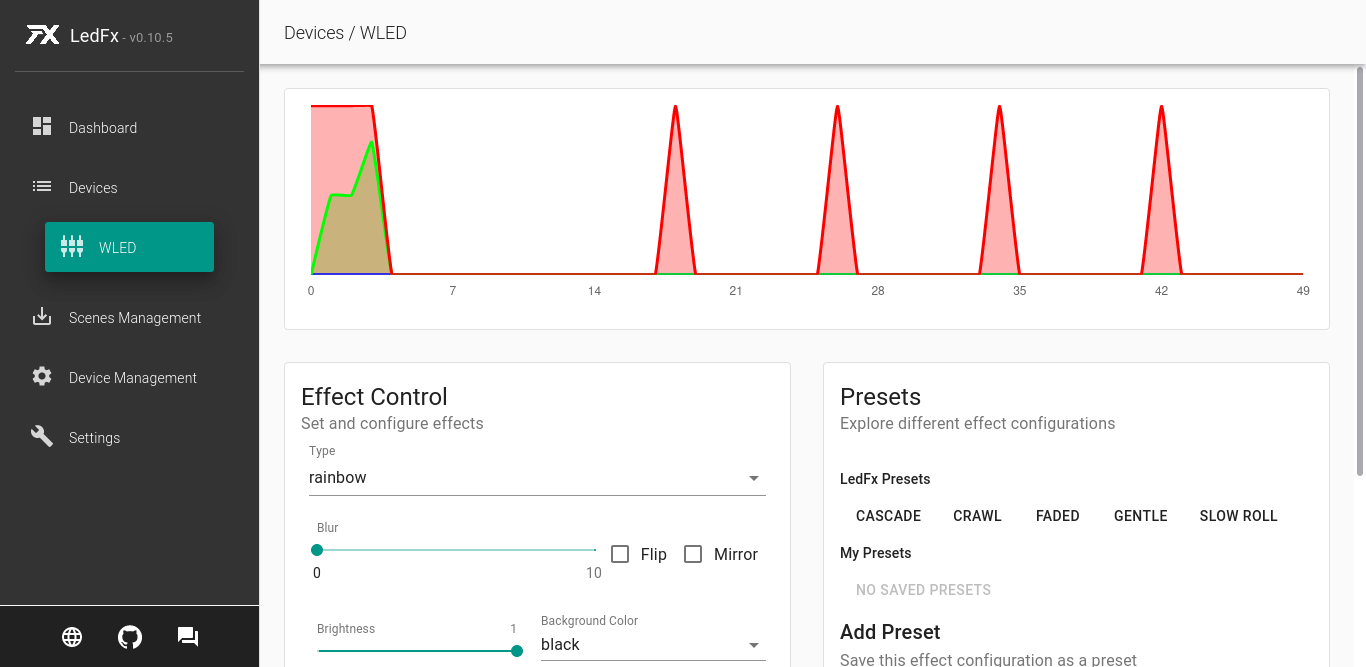
\includegraphics[width=\linewidth]{ledfx}
\end{frame}

\begin{frame}
  \large
  \textbf{کد برنامه اولیه}:
  \vspace{.7em}

  \lr{\url{github.com/mamins1376/espws2811}}
  \vspace{2em}

  \textbf{کد پایان‌نامه، مقاله در کنفرانس EM2021 و این ارائه}:
  \vspace{.7em}

  \lr{\url{github.com/mamins1376/arakut-defense}}
\end{frame}

\begin{frame}
  \Large ممنون از توجه شما.
  \par\vspace{2em}
  \Huge ?
\end{frame}

\end{document}
